\chapter{The Braid Group}\label{ch:braid_group}

\begin{definition}
    The \textit{configuration space} of $n$ ordered distinct points in the complex plane $\C$ is defined as $M_n = \left\{ \left( z_1,\dots,z_n \right)\in\C ; z_i\neq z_j,\forall i\neq j \right\}$. Alternatively, consider $\mathcal{D}$ to be the collection of all hyperplanes $H_{i,j}=\left\{ z_i=z_j \right\}\in\C^n$ for $1\leq i < j \leq n$. Then we can define $M_n = \C^n \setminus \mathcal{D}$.
\end{definition}

Note that $\left( z_1,z_2,z_3,\dots,z_n \right)$ and $\left( z_2,z_1,z_3,\dots,z_n \right)$ are different points in the configuration space $M_n$. Before studying the various interpretations of the braid group, we first define the braid group itself.

\begin{definition}
    The \textit{pure braid group} on $n$ strands, denoted $PB_n$, is the fundamental group of $M_n$. One can write $PB_n = \pi_1(M_n)$.
\end{definition}

\section{Visualization of pure braids}

We can think of a pure braid as a loop in $M_n$:
\begin{align*}
    \beta : \left[ 0,1 \right] &\to M_n \\
    t &\mapsto \beta(t) = \left( \beta_1(t),\beta_2(t),\dots,\beta_n(t) \right),
\end{align*}
with some base point. Conventionally, we define the base point as the $n$-tuple of integers $(1,2,3,\dots,n)\in \C^n$. Then a pure braid can be though of the motion of these points in the complex plane as $t$ ranges from 0 to 1 in which $\beta_i(t)$ is defined and $\beta_i(t)\neq \beta_j(t)$ for every $t\in[0,1]$ and $i\neq j\in\left\{ 1,2,\dots,n \right\}$. Because each $\beta_i$ is a loop, it must start and end at the point $i$ (e.g., $\beta_i(0)=\beta_i(1)=i$). Recall that the loops are actually equivalence classes of loops under homotopy. As a result, we can continuously deform the motion of the $n$ points while maintaining the same pure braid (up to equivalence) so long as we preserve the pairwise distinction of the points for all time $t\in[0,1]$.

A common visualization of pure braids is to plot the motion of the points in 3-dimensional space. For each $t\in [0,1]$, we draw the points $\left( \beta_i(t),t \right)$ in $\C\times[0,1]$ for every $i\in\left\{ 1,\dots,n \right\}$. The space $\C\times[0,1]$ can be thought of as a spacetime diagram, where the motion of the points is plotted in the complex plane at each time $t$, with the time being the vertical axis. The convention is to have $\C\times\left\{ 0 \right\}$ placed above $\C\times\left\{ 1 \right\}$, so that the motion of the points is plotted from top to bottom.

\missingfigure[figwidth=6cm]{Gonzalez Figure 1}

For every $i\in\left\{ 1,\dots,n \right\}$, the motion of a single point starting at $(i,0)$ and ending at $(i,1)$ is known as the $i$-th \textit{strand} of the pure braid. This can also be described by the $i$-th projection of the $n$-tuple $\beta(t)$. Thus, two braids are equivalent under homotopy if, for every moment of a continuous deformation of the $n$ strands in $\C\times [0,1]$, the (fixed) endpoints $((1,0),(2,0),\dots,(n,0))$ and $((1,1),(2,1),\dots,(n,1))$ are connected by strands that are pairwise disjoint where each strand intersects the plane $\C\times\left\{ t \right\}$ exactly once for every $t\in[0,1]$.

As pure braids are members of the pure braid group, multiplication is a well-defined operation. In the context of $M_n$, multiplication of pure braids involves the concatenation of loops. Visually, this is the process of stacking braids on top of each other, and then rescaling the time dimension so that $t$ ranges from 0 to 1.

\section{General braids}
In the previous section, we defined pure braids in which the endpoints of each strand are identical at the beginning and end of the motion. This notion generalizes to define (non-pure) braids. First, we define a more general configuration space than $M_n$. The symmetric group $S_n$ permutes the $n$ distinct points in $\C$. Then the \textit{configuration space of n unordered points in $\C$} is the quotient space $N_n = M_n/S_n$.

\begin{definition}
    The braid group on $n$ strands is the fundamental group of $N_n$, denoted $B_n = \pi_1(N_n)$.
\end{definition}

The visualization of a braid is the same as in the case of pure braids, only now the endpoints of each strand do not necessarily match the starting points. For example, the $i$-th strand may start at the point $(i,0)$ but end at the point $(j,1)$ for $i,j\in\left\{ 1,\dots,n \right\}$. The equivalence of strands is still defined as before under the homotopy of loops. Loop concatenation defines the multiplication of braids, as before.

\section{Standard generators of the braid group}\label{sec:std_gens}
Originally proposed by Artin~\cite{Artin1947}, each braid can be decomposed into a product of \textit{standard generators} of the braid group. When visualizing braids in $\R\times[0,1]$, a crossing of two strands is clearly indicated by one going over the other. Suppose each crossing occurs at a different time $t\in[0,1]$. Then by rescaling the time component of an arbitrary braid, we can deconstruct it into a stack of simple braids with only one crossing between neighboring strands per braid. Each single crossing of strands can be obtained by performing a transposition between neighboring endpoints of the strands.

\missingfigure[figwidth=6cm]{Gonzalez Figure 2}

For instance, swapping the endpoints of the $i$-th and $(i+1)$-th strands can be written as applying $\sigma_i$ to the identity braid (i.e., the braid that starts without any crossings of strands). It must be noted that there are two distinct ways to swap the endpoints of two strands. From a top-down perspective looking at the plane $\C\times\left\{ t \right\}$ for some time $t$, $\sigma_i$ swaps $(i,t)$ and $(i+1,t)$ in a clockwise rotation. The reverse of this operation (i.e., twisting the endpoints around in the counterclockwise direction) is denoted $\sigma_i^{-1}$. The standard generators of the braid group $B_n$ are defined as the set $\left\{ \sigma_1,\sigma_2,\dots,\sigma_{n-1} \right\}$. An arbitrary braid can be constructed by concatenating (or stacking) the simple braids made from the standard generators before rescaling the time coordinate to $[0,1]$.

\section{Automorphisms of the free group}\label{sec:Aut_Fn}

Consider the $n$-times punctured disk $\D_n$. The fundamental group of $\D_n$ involves loops that start and end at the same (fixed) base point in $\partial\D_n$. Up to homotopy, a clockwise-directional loop that encompasses the $i$-th hole in $\D_n$ corresponds to the $i$-th generator of the free group $F_n$ of rank $n$, which is illustrated in \cref{fig:Gen_on_Dn}. In fact, $\pi_1\left( \D_n \right) = F_n$. This equality allows us to define a representation of the braid group on $n$ strands as automorphisms of $F_n$.

\begin{figure}[htbp]
    \centering
    % Suggested circle radius >= 3 cm
% \usetikzlibrary{decorations.markings}
\def\circleRadius{3cm}
\def\sep{\circleRadius*0.175}

\newcommand{\drawloop}[3]{\draw[ultra thick, postaction={decorate}] (0,-\circleRadius) .. controls #1 .. node[pos=#3, left] {#2} (.0*\sep,-\circleRadius);}

\begin{tikzpicture}[decoration={markings, 
	mark= at position 0.75 with {\arrow{latex},sloped}}
] 
        \node[anchor=north west, font=\Large] at (-\circleRadius, \circleRadius) {$\D_n$};

        \draw[ultra thick] (0,0) circle (\circleRadius);
        \filldraw [black] 
                        (-\circleRadius + \sep,0) circle (2pt) node[above, yshift=.2*\sep] {$1$}
                        (\circleRadius - \sep,0) circle (2pt) node[above, yshift=.2*\sep] {$n$}
                        (0,0) circle (2pt) node[above, yshift=.2*\sep] {$i$};
        \path (-\circleRadius/2 + \sep/2,0) node {$\scalebox{1.5}{$\cdots$}$};
        \path (\circleRadius/2 - \sep/2,0) node {$\scalebox{1.5}{$\cdots$}$};

        \drawloop{(-.35*\circleRadius,0.4*\circleRadius) and  (.35*\circleRadius,0.4*\circleRadius)}{$x_i$}{.2}

        \drawloop{(-1.6*\circleRadius,0.37*\circleRadius) and  (-.65*\circleRadius,0.43*\circleRadius)}{$x_1$}{.1}
        
        \drawloop{(.65*\circleRadius,0.43*\circleRadius) and  (1.6*\circleRadius,0.37*\circleRadius)}{$x_n$}{.25}
        
        % base point for loop/arrow
        \filldraw [red] (0,-\circleRadius) circle (2pt);
\end{tikzpicture}

    \caption{For each $i\in\left\{ 1,\dots,n \right\}$, the clockwise-directional loop encircling the $i$-th hole in $\D_n$ corresponds to the $i$-th free generator of $F_n$ (i.e., $x_i$). The red dot indicates the (arbitrary) base point for the loops in $\pi_1(\D_n)$.}\label{fig:Gen_on_Dn}
\end{figure}

Each braid $\beta\in B_n$ is realized as an automorphism of $\pi_1(\D_n) = F_n$ (up to isotopy) where each loop $\gamma\in\pi_1(\D_n)$ is sent to another loop $\beta(\gamma)$. In other words, we have a representation of the braid group defined by
\begin{align}
    \rho: B_n &\to \aut{F_n} \\
    \beta &\mapsto \rho_\beta.
\end{align}
The action of $\beta$ on a loop $\gamma$ is defined by the rearrangements of the $n$ holes in $\D_n$, similar to the action of the standard generators of $B_n$ on the base points in $\C\times\left\{ 1 \right\}$. In terms of the standard generators of $B_n$, each $\sigma_i$ corresponds to switching the places of hole $i$ and hole $i+1$ by means of a clockwise rotation, as seen in \cref{fig:sigma_on_Dn}. This is identical to viewing the action of $\sigma_i$ on the base points (\cref{sec:std_gens}) from above, looking down on the $\C\times\left\{ t \right\}$-plane. As before, the inverse action $\iv{\sigma_i}$ is a counterclockwise rotation of the two adjacent holes $i$ and $i+1$ in $\D_n$. These actions respect the group operation of loop concatenation.

\colorbox{red}{A note on convention of directions/consistency up to inverses.}

% \begin{figure}[htbp]
%     \centering
%     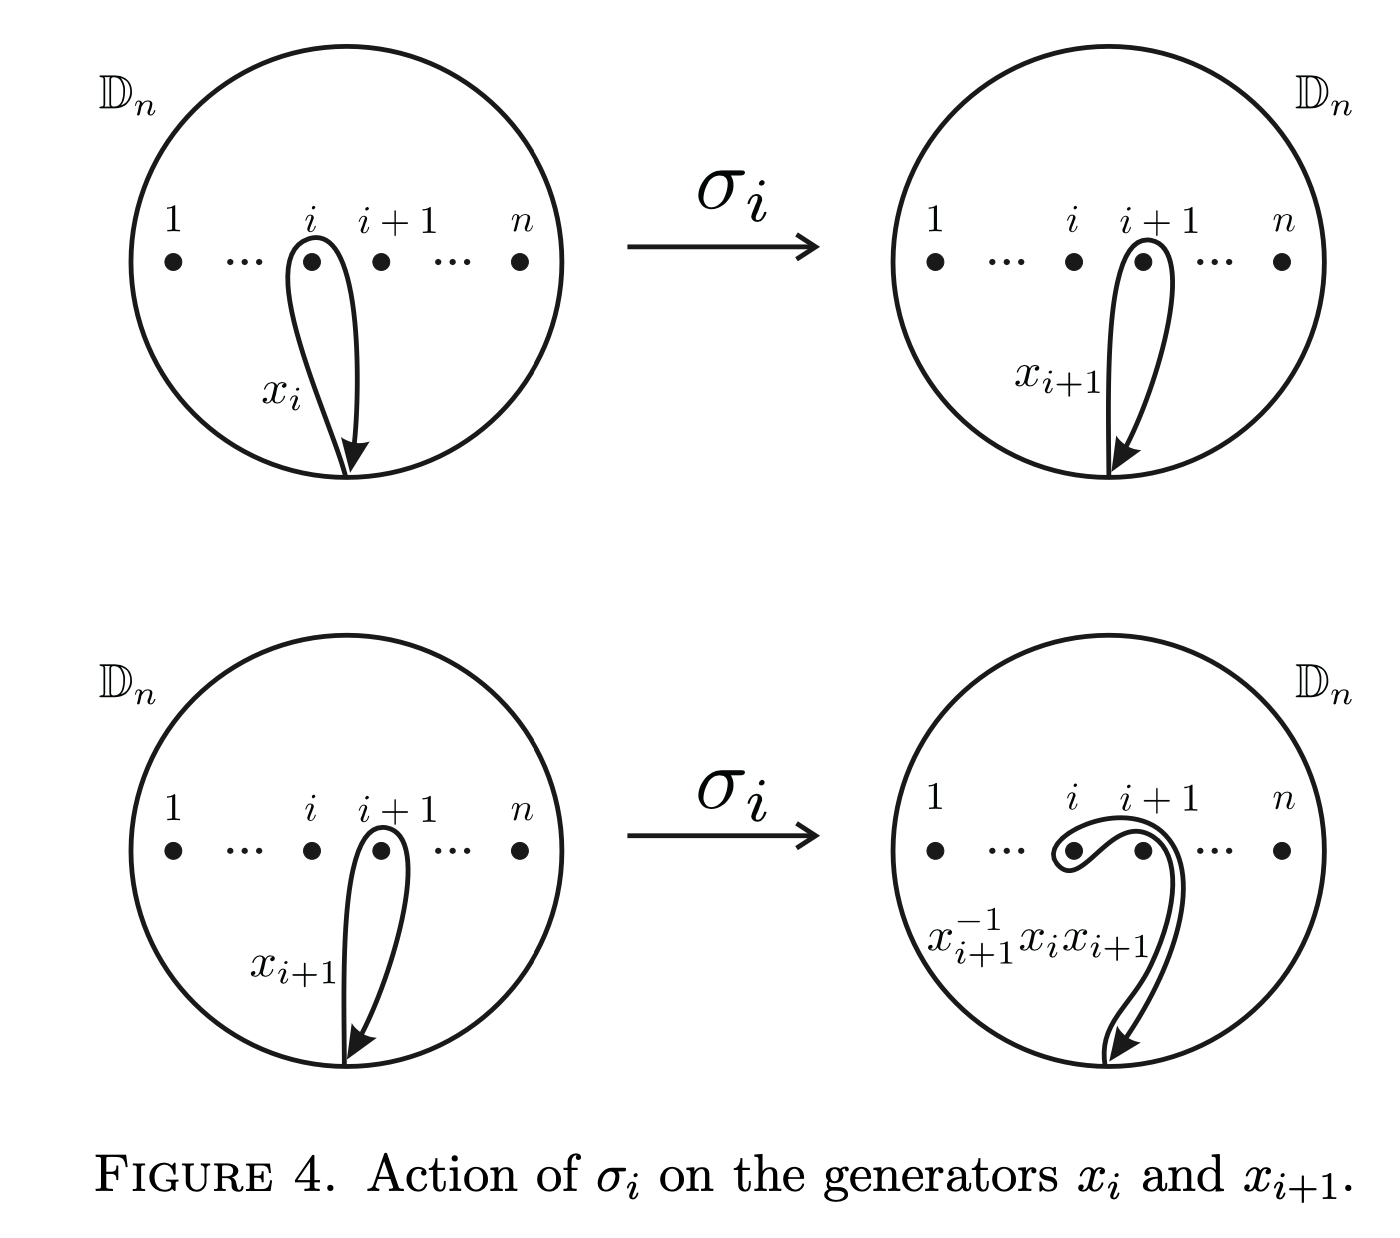
\includegraphics[width = .5\textwidth]{Gonzalez_Fig4_sigma_on_Dn.png}
%     \caption{\colorbox{red}{Gonzalez Figure 4}}\label{fig:sigma_on_Dn}
% \end{figure}

\begin{figure}[htbp]
    \centering
    \def\circleRadius{2.5cm}
\def\sep{\circleRadius*0.175}
\def\XOff{1.5*\circleRadius}
\def\YOff{-2.5*\circleRadius}

\pgfdeclarelayer{edgelayer}
\pgfdeclarelayer{nodelayer}
\pgfsetlayers{edgelayer,nodelayer,main}

\newcommand{\drawRegion}[3]{
        \begin{scope}[shift={#1}]
        \node[anchor=north west, font=\large] at (-\circleRadius, \circleRadius) {$\D_n$};

        \draw[ultra thick] (0,0) circle (\circleRadius);
        \filldraw [black] 
                (-\circleRadius + \sep,0) circle (2pt) node[above] {$1$}
                (\circleRadius - \sep,0) circle (2pt) node[above] {$n$}
                (-\sep,0) circle (2pt) node[above, yshift=.2*\sep] {$i$}
                (\sep,0) circle (2pt) node[above, yshift=.1*\sep] {$i+1$};
        \path (-\circleRadius/2,0) node {$\scalebox{1.5}{$\cdots$}$};
        \path (\circleRadius/2,0) node {$\scalebox{1.5}{$\cdots$}$};

        \ifx&#2&  % Check if #2 is empty
                % Do nothing if #2 is empty
        \else
                \draw[-latex, ultra thick] (0,-\circleRadius) .. controls #2 .. node[pos=0.1, left] {#3} (.05*\sep,-\circleRadius + 2.8452755906/2);
        \fi
        
        \filldraw [red] (0,-\circleRadius) circle (2pt);
        
        \end{scope}
}


\begin{tikzpicture}
        \drawRegion{(\XOff,0)}{(-1.425*\sep-.35*\circleRadius,0.39*\circleRadius) and  (-1.425*\sep+.35*\circleRadius,0.39*\circleRadius)}{$x_i$}
        
        \draw[-latex, ultra thick] (-\XOff + \circleRadius + 0.25cm, 0) -- node[above] {$\sigma_i$} (\XOff - \circleRadius - 0.25cm, 0);
        
        \drawRegion{(-\XOff,0)}{(1.3*\sep-.35*\circleRadius,0.39*\circleRadius) and  (1.3*\sep+.35*\circleRadius,0.39*\circleRadius)}{$x_{i+1}$}
        
        \drawRegion{(-\XOff,\YOff)}{(-1.425*\sep-.35*\circleRadius,0.39*\circleRadius) and  (-1.425*\sep+.35*\circleRadius,0.39*\circleRadius)}{$x_i$}

        \draw[-latex, ultra thick] (-\XOff + \circleRadius + 0.25cm, \YOff) -- node[above] {$\sigma_i$} (\XOff - \circleRadius - 0.25cm, \YOff);
        
        % \drawRegion{(\XOff,\YOff)}{}{}

        \begin{scope}[shift={(\XOff,\YOff)}]
                \node[anchor=north west, font=\large] at (-\circleRadius, \circleRadius) {$\D_n$};
        
                \draw[ultra thick] (0,0) circle (\circleRadius);
                \filldraw [black] 
                        (-\circleRadius + \sep,0) circle (2pt) node[above] {$1$}
                        (\circleRadius - \sep,0) circle (2pt) node[above] {$n$}
                        (-\sep,0) circle (2pt) node[above, yshift=.45*\sep] {$i$}
                        (\sep,0) circle (2pt) node[above, yshift=.3*\sep] {$i+1$};
                \path (-\circleRadius/2,0) node {$\scalebox{1.5}{$\cdots$}$};
                \path (\circleRadius/2,0) node {$\scalebox{1.5}{$\cdots$}$};
        
                \filldraw [red] (0,-\circleRadius) circle (2pt);

                \begin{pgfonlayer}{nodelayer}
                        \node (0) at (-1.5*\sep,.35*\sep ) {};
                        \node (1) at (0, -\circleRadius) {};
                        \node (2) at (1.5*\sep, -1.5*\sep) {$x_i x_{i+1}\iv{x_i}$};
                        \node (3) at (1.25*\sep, -.25*\sep) {};
                        \node (4) at (-.5*\sep, .35*\sep) {};
                        \node (5) at (.05*\sep, -\circleRadius + 2.8452755906/2) {};
                \end{pgfonlayer}
                \begin{pgfonlayer}{edgelayer}
                        \draw [in=105, out=-120, looseness=0.50, ultra thick] (0.center) to (1.center);
                        \draw [in=60, out=30, looseness=0.85, ultra thick] (3.center) to (0.center);
                        \draw [in=-150, out=-15, looseness=0.50, ultra thick] (4.center) to (3.center);
                        \draw [latex-, in=165, out=85, ultra thick] (5.center) to (4.center);
                \end{pgfonlayer}

                % \foreach \point in {0,1,3,4,5} {
                %         \fill[red] (\point) circle (2pt);
                %         \node[above right] at (\point) {\point};
                % }
        \end{scope}
        
        \draw[-latex, ultra thick] (-\XOff + \circleRadius + 0.25cm, 0) -- node[above] {$\sigma_i$} (\XOff - \circleRadius - 0.25cm, 0);
\end{tikzpicture}
    \caption{The action of $\sigma_i$ on the generators $x_i$ and $x_{i+1}$ as described by \cref{eq:rho_i,eq:rho_ip1,eq:rho_j}. The image of $x_i$ under $\sigma_i$ is verified visually in \cref{fig:sigma_on_x_i}}\label{fig:sigma_on_Dn}
\end{figure}

The automorphism $\rho_\beta$ is most simply defined in terms of the action of the standard generators of $B_n$ on the generators $x_1,\dots,x_n$ of $F_n$ (visualized as loops in $\D_n$). For each $i$, it follows that
\begin{align}
    &\rho_{\sigma_i}(x_{i}) = x_{i}x_{i+1} \iv{x_{i}}, \label{eq:rho_i}\\
    &\rho_{\sigma_i}(x_{i+1}) = x_{i}, \label{eq:rho_ip1}\\
    &\rho_{\sigma_i}(x_j) = x_j, \textrm{ for } j\neq i,i-1.\label{eq:rho_j}
\end{align}
Clearly, any two loops that are separated by at least one puncture will not interact while performing $\sigma_i$. The relations for adjacent loops can be verified graphically as illustrated in \cref{fig:sigma_on_Dn,fig:sigma_on_x_i}.
\begin{figure}[htbp]
    \centering
    \def\circleRadius{2.5cm}
\def\sep{\circleRadius*0.175}
\def\XOff{1.5*\circleRadius}
\def\YOff{-2.5*\circleRadius}

\usetikzlibrary{decorations.markings}

\pgfdeclarelayer{edgelayer}
\pgfdeclarelayer{nodelayer}
\pgfsetlayers{edgelayer,nodelayer,main}

\newcommand{\drawRegion}[3]{
        \begin{scope}[shift={#1}]
        \node[anchor=north west, font=\large] at (-\circleRadius, \circleRadius) {$\D_n$};

        \draw[ultra thick] (0,0) circle (\circleRadius);
        \filldraw [black] 
                (-\circleRadius + \sep,0) circle (2pt) node[above] {$0$}
                (\circleRadius - \sep,0) circle (2pt) node[above] {$n$}
                (-\sep,0) circle (2pt) node[above, yshift=.2*\sep] {$i$}
                (\sep,0) circle (2pt) node[above, yshift=.1*\sep] {$i+1$};
        \path (-\circleRadius/2,0) node {$\scalebox{1.5}{$\cdots$}$};
        \path (\circleRadius/2,0) node {$\scalebox{1.5}{$\cdots$}$};

        \filldraw [red] (0,-\circleRadius) circle (2pt);

        \ifx&#2&  % Check if #2 is empty
                % Do nothing if #2 is empty
        \else
                \draw[-latex, ultra thick] (0,-\circleRadius + 2.8452755906/2) .. controls #2 .. node[pos=0.1, left] {#3} (.05*\sep,-\circleRadius + 2.8452755906/2);
        \fi
        \end{scope}
}

\newcommand{\drawloop}[4]{\draw[ultra thick, postaction={decorate}, decoration={markings, mark= at position 0.75 with {\arrow{latex},sloped}}, #2] (0,-\circleRadius + 2.8452755906/2) .. controls #1 .. node[pos=#4, left] {#3} (.05*\sep,-\circleRadius + 2.8452755906/2);}

\newcommand{\rdrawloop}[4]{\draw[ultra thick, postaction={decorate}, decoration={markings, mark= at position 0.25 with {\arrowreversed{latex},sloped}}, #2] (0,-\circleRadius + 2.8452755906/2) .. controls #1 .. node[pos=#4, left] {#3} (.05*\sep,-\circleRadius + 2.8452755906/2);}


\begin{tikzpicture}
        \begin{scope}[shift={(-\XOff,0)}]
                \node[anchor=north west, font=\large] at (-\circleRadius, \circleRadius) {$\D_n$};
        
                \draw[ultra thick] (0,0) circle (\circleRadius);
                \filldraw [black] 
                        (-\circleRadius + \sep,0) circle (2pt) node[above] {$0$}
                        (\circleRadius - \sep,0) circle (2pt) node[above] {$n$}
                        (-\sep,0) circle (2pt) node[above, yshift=.2*\sep] {$i$}
                        (\sep,0) circle (2pt) node[above, yshift=.25*\sep] {$i+1$};
                \path (-\circleRadius/2,0) node {$\scalebox{1.5}{$\cdots$}$};
                \path (\circleRadius/2,0) node {$\scalebox{1.5}{$\cdots$}$};
        
                \filldraw [red] (0,-\circleRadius) circle (2pt);

                \begin{pgfonlayer}{nodelayer}
                        \node (0) at (.7*\sep,-.5*\circleRadius ) {};
                        \node (1) at (0, -\circleRadius + 2.8452755906/2) {};
                        \node (2) at (.5*\circleRadius, -2*\sep) {$\color{NavyBlue} x_{i+1}$};
                        \node (3) at (.9*\sep, .5*\sep) {};
                        \node (4) at (1.75*\sep, -.5*\circleRadius) {};
                        \node (5) at (.05*\sep, -\circleRadius + 2.8452755906/2) {};
                \end{pgfonlayer}
                \begin{pgfonlayer}{edgelayer}
                        \draw [in=30, out=-90, looseness=0.50, ultra thick, NavyBlue] (0.center) to (1.center);
                        \draw [in=90, out=-150, looseness=0.85, ultra thick, NavyBlue] (3.center) to (0.center);
                        \draw [in=20, out=80, looseness=0.50, ultra thick, NavyBlue, postaction={decorate}, decoration={markings, mark= at position .5 with {\arrowreversed{latex},sloped}}] (4.center) to (3.center);
                        \draw [in=-100, out=10, ultra thick, NavyBlue] (5.center) to (4.center);
                \end{pgfonlayer}
                
                % \foreach \point in {0,1,3,4,5} {
                %         \fill[red] (\point) circle (2pt);
                %         \node[above right] at (\point) {\point};
                % }

                \rdrawloop{(-1.4*\sep-.65*\circleRadius,0.7*\circleRadius) and  (-1.4*\sep+.55*\circleRadius,0.7*\circleRadius)}{purple}{$\iv{x_i}$}{.45}

                \drawloop{(-1.4*\sep-.35*\circleRadius,0.39*\circleRadius) and  (-1.4*\sep+.35*\circleRadius,0.39*\circleRadius)}{OliveGreen}{$x_i$}{.1}

        \end{scope}

        \begin{scope}[shift={(\XOff,0)}]
                \node[anchor=north west, font=\large] at (-\circleRadius, \circleRadius) {$\D_n$};
        
                \draw[ultra thick] (0,0) circle (\circleRadius);
                \filldraw [black] 
                        (-\circleRadius + \sep,0) circle (2pt) node[above] {$0$}
                        (\circleRadius - \sep,0) circle (2pt) node[above] {$n$}
                        (-\sep,0) circle (2pt) node[above, yshift=.3*\sep] {\small$i$}
                        (\sep,0) circle (2pt) node[above, xshift=0*\sep, yshift=.15*\sep] {\small$i+1$};
                \path (-\circleRadius/2,0) node {$\scalebox{1.5}{$\cdots$}$};
                \path (\circleRadius/2,0) node {$\scalebox{1.5}{$\cdots$}$};
        
                \filldraw [red] (0,-\circleRadius) circle (2pt);
                
                \begin{scope}[shift={(-.25*\sep,0)}]
                                \begin{pgfonlayer}{nodelayer}
                                \node (0) at (-1.75*\sep,-.15*\circleRadius ) {};
                                \node (1) at (.25*\sep, -\circleRadius + 2.8452755906/2) {};
                                % \node (2) at (.5*\circleRadius, -2*\sep) {$x_i x_{i+1}\iv{x_i}$};
                                \node (3) at (0*\sep, 1.5*\sep) {};
                                \node (4) at (2*\sep, -.05*\circleRadius) {};
                                \node (5) at (0*\sep, 0*\circleRadius) {};
                                \node (6) at (-1.2*\sep, .4*\sep) {};
                                \node (7) at (.3*\sep, -\circleRadius + 2.8452755906/2) {};

                                \node (ip1) at (2.5*\sep, -1.15*\sep) {$\color{NavyBlue} x_{i+1}$};
                                \node (i) at (-.4*\circleRadius, -2*\sep) {$\color{OliveGreen} x_{i}$};
                                \node (iiv) at (.1*\circleRadius, -3*\sep) {$\color{purple} \iv{x_{i}}$};
                        \end{pgfonlayer}
                        \begin{pgfonlayer}{edgelayer}
                                \draw [in=150, out=-90, looseness=0.50, ultra thick, OliveGreen] (0.center) to (1.center);
                                \draw [latex-, in=100, out=180, looseness=0.95, ultra thick, OliveGreen] (3.center) to (0.center);
                                \draw [in=0, out=90, looseness=0.9, ultra thick, NavyBlue] (4.center) to (3.center);
                                \draw [latex-, in=-100, out=-50, looseness=.9, ultra thick, NavyBlue] (5.center) to (4.center);
                                \draw [in=60, out=100, looseness=.9, ultra thick, purple] (5.center) to (6.center);
                                \draw [-latex, in=100, out=-110, looseness=.9, ultra thick, purple] (6.center) to (7.center);
                        \end{pgfonlayer}
                \end{scope}
                
                \foreach \point in {3,5} {
                                \fill[red] (\point) circle (1.5pt);
                                % \node[above right] at (\point) {\point};
                        }

                % \foreach \point in {0,1,3,4,5,6,7} {
                %         \fill[red] (\point) circle (1.5pt);
                %         \node[above right] at (\point) {\point};
                % }
        \end{scope}

        \begin{scope}[shift={(\XOff,\YOff)}]
                \node[anchor=north west, font=\large] at (-\circleRadius, \circleRadius) {$\D_n$};
        
                \draw[ultra thick] (0,0) circle (\circleRadius);
                \filldraw [black] 
                        (-\circleRadius + \sep,0) circle (2pt) node[above] {$0$}
                        (\circleRadius - \sep,0) circle (2pt) node[above] {$n$}
                        (-\sep,0) circle (2pt) node[above, yshift=.45*\sep] {$i$}
                        (\sep,0) circle (2pt) node[above, yshift=.3*\sep] {$i+1$};
                \path (-\circleRadius/2,0) node {$\scalebox{1.5}{$\cdots$}$};
                \path (\circleRadius/2,0) node {$\scalebox{1.5}{$\cdots$}$};
        
                \filldraw [red] (0,-\circleRadius) circle (2pt);

                \begin{pgfonlayer}{nodelayer}
                        \node (0) at (-1.5*\sep,.35*\sep ) {};
                        \node (1) at (0, -\circleRadius + 2.8452755906/2) {};
                        \node (2) at (1.5*\sep, -1.5*\sep) {$x_i x_{i+1}\iv{x_i}$};
                        \node (3) at (1.25*\sep, -.25*\sep) {};
                        \node (4) at (-.5*\sep, .35*\sep) {};
                        \node (5) at (.05*\sep, -\circleRadius + 2.8452755906/2) {};
                \end{pgfonlayer}
                \begin{pgfonlayer}{edgelayer}
                        \draw [in=105, out=-120, looseness=0.50, ultra thick] (0.center) to (1.center);
                        \draw [in=60, out=30, looseness=0.85, ultra thick] (3.center) to (0.center);
                        \draw [in=-150, out=-15, looseness=0.50, ultra thick] (4.center) to (3.center);
                        \draw [latex-, in=165, out=85, ultra thick] (5.center) to (4.center);
                \end{pgfonlayer}

        \end{scope}
        
        \draw[latex-latex, ultra thick] (-\XOff + \circleRadius + 0.25cm, 0) -- node[above] {\footnotesize Homotopic} node[below] {\tiny (Loop Concatenation)} (\XOff - \circleRadius - 0.25cm, 0);
        
        \draw[latex-latex, ultra thick] (\XOff, -\circleRadius - 0.1cm) -- (\XOff, \YOff+\circleRadius + 0.1cm);
\end{tikzpicture}
    \caption{Up to homotopy, the product $x_i x_{i+1} \iv{x_i}$ is visualized as the concatenation of the loops $x_i,x_{i+1},\iv{x_i}\in\pi_1(\D_n)$. In the top right diagram, small red dots are used indicate the (homotopically deformed) points of concatenation.}\label{fig:sigma_on_x_i}
\end{figure}

For any $\sigma_i$, $\rho_{\iv{\sigma_i}}$ is well-defined. It follows that for any braid $\beta\in B_n$, we can decompose $\rho_\beta$ the composition of the automorphisms of the standard generators $\sigma_1,\dots,\sigma_{n-1}$ and their inverses that make up $\beta$. 

Notice that for any $\sigma_i$, $\rho_{\sigma_i}(x_1\cdots x_n) = x_1\cdots x_n$. This is because the loop $x_1\cdots x_n$ in $\D_n$, encompassing all holes, is parallel to the boundary $\partial\D_n$. Thus, the action of $\sigma_i$ on $x_1\cdots x_n$ is trivial does not affect the structure of the loop up to isotopy. More generally, this implies that $\rho_\beta(x_1\cdots x_n) = x_1\cdots x_n$ for any $\beta\in B_n$. Paired with the observation that every generator is conjugate to another, Artin~\cite{Artin1947} showed that this is a necessary and sufficient condition for $\rho_\beta$ to be an automorphism of $F_n$.

\begin{theorem}
    An automorphism $f\in\aut{F_n}$ is equal to $\rho_\beta$ for some $\beta\in B_n$ if and only if
    \begin{enumerate}
        \item $f(x_i)$ is a conjugate of some $x_j$ for every $i\in\left\{ 1,\dots,n \right\}$, and
        \item $f(x_1\cdots x_n) = x_1\cdots x_n$.
    \end{enumerate}
\end{theorem}

In this interpretation of the braid group, we can express $B_n$ in terms of the standard generators:
\begin{equation}
    B_n = \left\langle \sigma_1,\dots,\sigma_{n-1} \;\middle|\;
    \begin{aligned}
        \sigma_i\sigma_j &= \sigma_j\sigma_i, & |i-j|&>1 \\
        \sigma_i\sigma_{i+1}\sigma_i &= \sigma_{i+1}\sigma_i\sigma_{i+1}, & |i-j|&=1
    \end{aligned}
    \right\rangle.
\end{equation}
The first condition that the standard generators commute if $|i-j|>1$ is easily verified by looking at the graphic of \cref{fig:sigma_on_x_i} in describing the property of the automorphism $\rho_{\sigma_i}(\sigma_j) = \sigma_j$. This follows by the fact that if two holes are non-adjacent, then the actions of $\sigma_i$ and $\sigma_j$ are mutually exclusive and thus commutative. The second condition on the standard generators is most easily verified in \cref{fig:YB_criterion_verification} by looking at the corresponding braids in $\R\times[0,1]$.
\begin{figure}[htbp]
    \centering
    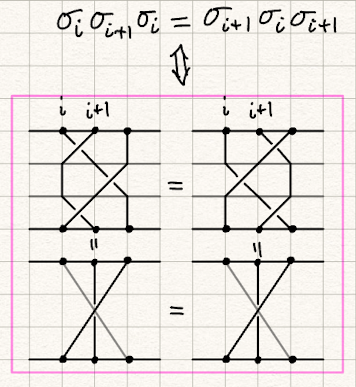
\includegraphics[width = .5\textwidth]{sketch_YB_citerion_verification.png}
    \caption{\colorbox{red}{Grayed-out strand indicates that it is behind all other strands.}}\label{fig:YB_criterion_verification}
\end{figure}

\section{The Burau Representation}
In the previous section, we defined a representation of the braid group $B_n$ as automorphisms of the free group $F_n$. This representation is clearly nonabelian. Likewise, the Artin generators of $B_n$ are nonabelian. Suppose we wish to abelianize the braid group. The details of the abelianization of $B_n$ would require a quotient by the commutator $\left[ a,b \right]=ab\iv{a}\iv{b}$.

Sparing the details, let $B_{n,ab} = B_n/\left[ B_n,B_n \right]$ be the abelianization of $B_n$, where $\left[ B_n,B_n \right]=\left\{ \left[ \beta_1,\beta_2 \right]\st\beta_1,\beta_2\in B_n \right\}$ is the commutator subgroup of $B_n$. Then, under the representation $\rho$ from \cref{sec:Aut_Fn}, the abelianization of \cref{eq:rho_i,eq:rho_ip1,eq:rho_j} become
\begin{align}
    x_i &\xmapsto{\sigma_i} \cancel{x_i} + x_{i+1} - \cancel{x_i} = x_{i+1} = \rho_{\iv{\sigma_i}}(x_i), \\
    x_{i+1} &\xmapsto{\sigma_i} x_i, \\
    x_j &\xmapsto{\sigma_i} x_j, \textrm{ for } j\neq i,i-1,
\end{align}
for each $i$. Thus, the generator $\sigma_i=\iv{\sigma_i}$, and corresponds to a transposition permutation in the symmetric group $S_n$. It follows that $B_{n,ab}\iso S_n$. In this current construction, the abelianization of the braid group results in a loss of complexity. This raises the question whether there exists such a reframing of the braid group that allows an abelian operation on the free generators while preserving the inequivalence of the Artin generators with their inverses.

First, we define a topological space that will aid in the desired construction.
\begin{definition}
    Let $X$ be a topological space. A \textit{covering} of $X$ is a space $\widetilde{X}$ together with a continuous map $p:\widetilde{X}\to X$ such that, for every $x\in X$, there exists a path-connected open neighborhood $U$ containing $x$ such that $\iv{p}(U)$ is a disjoint union of open sets in $\widetilde{X}$ where each component of $\iv{p}(U)$ is mapped homeomorphically onto $U$ by $p$. Each component of $\iv{p}(U)$ is called a \textit{sheet} of the covering, where the $i$-th sheet is denoted by $\sheet{X}{i}$, and total the number of sheets in $\iv{p}(U)$ is called the \textit{degree} of the covering.
\end{definition}

\begin{example}
    One of the simplest examples of a covering space is the covering of the circle $S^1$ by the real line by the parameterization map $p:\R\to S^1$ defined by $p(t)=\left( \cos t,\sin t \right)$. Clearly, there are infinitely many sheets in this covering.
\end{example}

\begin{example}
    A similar example is the covering of the circle $S^1$ through $p:\left[ 0,1 \right]\to S^1$ defined by $p(t) = e^{2\pi it}$. This defines a one-degree covering of $S^1$. If we instead let our domain be $\left[ 0,2 \right]$, then we have a two-degree covering of $S^1$.
\end{example}

With this topological tool, we construct a countably infinite-degree covering of of the punctured disk $\D_n$, denoted $\widetilde{\D}_n$, which can be visualized as an infinite stack of copies of $\D_n$, with a slight modification to be explained shortly. Let $\sheet{\D}{n,i}$ denote the $i$-th sheet of $\widetilde{\D}_n$, and consider the base sheet our covering to be $\sheet{\D}{n,0}$.

We start this construction with a countably infinite stack of copies of $\D_n$. Then, for every $i\in\Z$, for each of the $n$ punctures on $\sheet{\D}{n,i}$, apply a cut from the hole to some point on the boundary of $\sheet{\D}{n,i}$, as illustrated in \cref{fig:D3_cuts}. Each cut results in two edges, which will be referred to as the left edge and the right edge. Through a homeomorphic deformation, connect the left edge of $\sheet{\D}{n,i}$ to the corresponding right edge of $\sheet{\D}{n,i+1}$, and the right edge of $\sheet{\D}{n,i}$ to the left edge of $\sheet{\D}{n,i-1}$, for every cut on every sheet.

\begin{figure}[htbp]
    \centering
    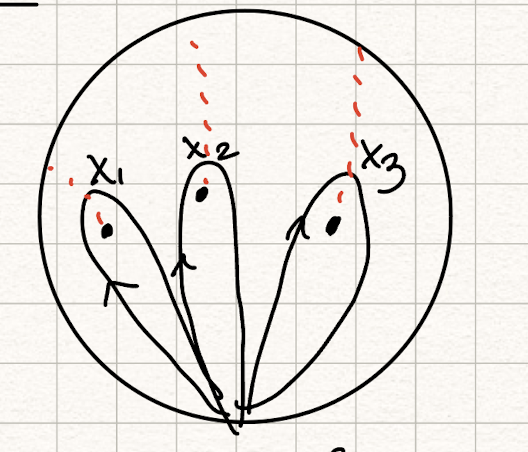
\includegraphics[width=.3\textwidth]{D3_cuts.png}
    % \input{TikZ/D3_covering.tikz}
    \caption{\colorbox{red}{CAPTION} Don't show the loops, and maybe actually show the cuts separated, and make sure to indicate/label the left and right edges.}\label{fig:D3_cuts}
\end{figure}

Now, when viewing a single sheet, say $\sheet{\D}{n,0}$, from above as in \cref{fig:D3_cuts}, when a loop with base point $\tilde{\zeta}_0$ passes through a cut from the left, it traverses up to the next sheet, and ends at the base point $\tilde{\zeta}_1$. Similarly, a loop passing through a cut from the right ends at the base point $\tilde{\zeta}_{-1}$, on the sheet $\sheet{\D}{n,-1}$ below $\sheet{\D}{n,0}$. To keep track of the starting sheet of a loop, we use a free parameter $t$. For example, a loop $\gamma$ that starts on $\sheet{\D}{n,j}$ would be written $t^j \gamma$, for $j\in\Z$. Notice that the substitution of a complex number for the free parameter $t$ results in a possibly finite degree covering. As an example, if we set $t$ to an $n$-th root of unity, then we obtain an $n$-th degree covering of $\D_n$. For the purposes of this construction, we will keep $t$ as a free parameter for now. The following example describes the action of the standard generators of $B_3$ on the covering space $\widetilde{\D}_3$.

\begin{example}\label{ex:Burau_D3}
    Consider the case when $n=3$. Then we have the corresponding covering space $\widetilde{\D}_3$ of $\D_3$. The action of the standard generators of $B_3$ in $\pi_1(\D_3)$ is known, and can be visualized in \cref{fig:sigma_on_Dn}. In the context of the covering space $\widetilde{\D}_3$, the action of each of the three generators $\sigma_1,\sigma_2,\sigma_3$ is understood by reducing the visuals to only the base points on each sheet and the loops themselves. This can be seen in \cref{fig:Burau_D3} for the case of $\sigma_1$.
    
    \begin{figure}[htbp]
        \centering
        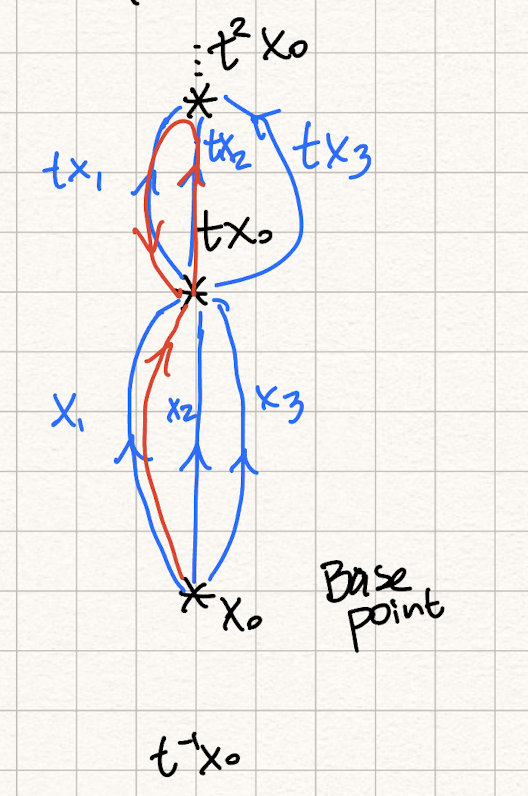
\includegraphics[width = .3\textwidth]{Burau_D3.png}
    %     % \input{TikZ/D3_covering.tikz}
        \caption{\colorbox{red}{CAPTION}}\label{fig:Burau_D3}
    \end{figure}

    Now, the loop concatenation is abelian, where \cref{eq:rho_i,eq:rho_ip1,eq:rho_j} become
    \begin{align}
        x_1 \xmapsto{\sigma_1} x_1 + tx_2 - tx_1 &= (1-t)x_1 + tx_2, \\
        x_{2} &\xmapsto{\sigma_1} x_1, \\
        x_3 &\xmapsto{\sigma_1} x_3.
    \end{align}
    Consider the vector $\begin{bmatrix}
        x_1 \\ x_2 \\ x_3
    \end{bmatrix}$. Then the action of $\sigma_1$ on the loops $x_1$ and $x_2$ is realized by the matrix $\begin{bmatrix}
        1-t & t & 0 \\ 1 & 0 & 0 \\ 0 & 0 & 1
    \end{bmatrix}$ since
    \begin{equation}
        \begin{bmatrix}
            1-t & t & 0 \\ 1 & 0 & 0 \\ 0 & 0 & 1
        \end{bmatrix}\begin{bmatrix}
            x_1 \\ x_2 \\ x_3
        \end{bmatrix} = \begin{bmatrix}
            (1-t)x_1 + tx_2 \\ x_1 \\ x_3
        \end{bmatrix}.
    \end{equation}
    The action of $\sigma_2$ is obtained similarly, where
    \begin{equation}
        \sigma_2 \mapsto \begin{bmatrix}
            1 & 0 & 0 \\ 0 & 1-t & t \\ 0 & 1 & 0
        \end{bmatrix}.
    \end{equation}
    Notice that these matrices have entries in the ring of Laurent polynomials, $\Lambda=\Z[t,\iv{t}]$.
\end{example}

Clearly, the result from \cref{ex:Burau_D3} generalizes to the case of braids on $n$ strands. Fix $n>1$. Let $I_k$ denote the $k\times k$ dimensional identity matrix, and let
\begin{equation}
    U=\begin{bmatrix}
        1-t & t \\ 1 & 0
    \end{bmatrix}.
\end{equation} 
For $i\in\left\{ 1,\dots,n-1 \right\}$, the action of $\sigma_i$ on $\pi_1\left( \widetilde{\D}_n \right)$ is realized as an $n\times n$ matrix with entries in $\Lambda = \Z[t,\iv{t}]$. 

The Burau representation of $B_n$ is then defined by:
\begin{align}
    \psi_n:B_n&\to\textrm{GL}_n(\Lambda) \\
    \sigma_i &\mapsto \begin{bmatrix}
        I_{i-1} & 0 & 0 \\
        0 & U & 0 \\
        0 & 0 & I_{n-i-1}
    \end{bmatrix}.
\end{align}
\colorbox{red}{Show invertible/inverse?}

The Burau representation need only be defined on the standard generators, since any braid $\beta\in B_n$ decomposes into a product of $\sigma_1,\dots,\sigma_{n-1}$ and their inverses. Notice that if we set $t\to 1$, we recover the defining representation of $S_n$, as expected when we use a degree 1 covering space of $\D_n$ and force the action of the generators to be abelian. Furthermore, by direct computation, it follows that
\begin{align}
    \psi_n(\sigma_i)\psi_n(\sigma_j) &= \psi_n(\sigma_j)\psi_n(\sigma_i) \textrm{ for } |i-j|>1, \\
    \psi_n(\sigma_i)\psi_n(\sigma_{i+1})\psi_n(\sigma_i) &= \psi_n(\sigma_{i+1})\psi_n(\sigma_i)\psi_n(\sigma_{i+1}) \textrm{ for } |i-j|=1.
\end{align}